
%%
%% nb: use pdflatex to create pdf file with hyperlinks
%%

%% =====================================================================
%% DOCUMENT DATA
%% =====================================================================

\documentclass[11pt]{article}

\title{OpenCCG Realizer Manual}
\author{Michael White}


%% =====================================================================
%% PACKAGES
%% =====================================================================

\usepackage{openccg} % for hlds/ccg
\usepackage{graphicx} % for figs
\usepackage{gb4e} % for examples
%\usepackage{cgmacros,hylo,ccg} % for hlds/ccg

\usepackage[
  colorlinks=true, linkcolor=blue, citecolor=blue, urlcolor=blue,
  pdfstartview=FitH,
  pdftitle={OpenCCG Realizer Manual},
  pdfauthor={Michael White}
]{hyperref}

%\usepackage{mathptmx}

%% listing settings 
%% nb: not crazy about font, esp that bold not working with keywords
\usepackage{listings,color}
\lstset{language=Java,basicstyle=\ttfamily\footnotesize,keywordstyle=\underline,commentstyle=\itshape\color{blue}}
%basicstyle=\ttfamily\small

%% =====================================================================
%% NEW COMMANDS
%% =====================================================================

%\newcommand{\occg}{\textsf{OpenCCG}}
\newcommand{\occg}{OpenCCG}
\newcommand{\tccg}{\textsf{tccg}}
\newcommand{\ccgrz}{\textsf{ccg-realize}}
\newcommand{\ccgtest}{\textsf{ccg-test}}

\newcommand{\code}[1]{\texttt{#1}} %\small 
\newcommand{\eref}[2][]{(\ref{ex:#2}#1)} % ref to examples
\newcommand{\secref}[1]{Section~\ref{sec:#1}} % ref to sections
\newcommand{\figref}[1]{Figure~\ref{fig:#1}} % ref to figures
\newlength{\mytablen} % for indenting in terms
\newcommand{\mytab}[1]{
  \settowidth{\mytablen}{\ensuremath{#1}}
  \mbox{\hspace{\mytablen}}
}
\newcommand{\xor}{~\underline{\vee}~}
\newcommand{\shared}[1]{\fbox{\ensuremath{#1}}}
\newcommand{\alt}[1]{\mathsf{alt}_{#1}}
\newcommand{\opt}[1]{\mathsf{opt}_{#1}}
 
%% =====================================================================
%% DOCUMENT BODY
%% =====================================================================

\begin{document}

\thispagestyle{empty}
\maketitle
\tableofcontents
%\listoftables
\listoffigures
\newpage


%% to do:
%% making an n-gram model
%% DLFs

\section{About this manual}

This manual is a programmer's guide to using the \occg\ surface realizer
in Java applications. You can download and install \occg\ from its
website, \url{http://openccg.sourceforge.net}. Once you've unpacked the
archive, have a look at the \texttt{README} file for installation
instructions. For a brief introduction to writing grammars for \occg,
see the ``rough guide'' in \texttt{docs/grammars-rough-guide.pdf}.


\section{About the OpenCCG realizer}
\label{overview}

The OpenCCG realizer
\cite{White/Baldridge:2003,White-RLAC:2004,White-INLG:2004,White-ACLSoft:2005}
is an open source surface realizer for Steedman's
\cite{Steedman-LI:2000,Steedman:SynProc} Combinatory Categorial Grammar
(CCG), including the multi-modal extensions to CCG devised by Baldridge
and Kruijff \cite{Baldridge:PhD,Baldridge/Kruijff:2003}.

Like other chart realizers
\cite{Kay:1996,Shemtov:PhD,Carroll-and-co:1999,Bob-Moore:2002}, the
OpenCCG realizer takes as input a logical form specifying the
propositional meaning of a sentence, and returns one or more surface
strings that express this meaning according to the lexicon and grammar.
A distinguishing feature of OpenCCG is that it implements a hybrid
symbolic-statistical chart realization algorithm that combines (1) a
theoretically grounded approach to syntax and semantic composition, with
(2) the use of integrated language models for making choices among the
options left open by the grammar, thereby reducing the need for
hand-crafted rules.

To allow language models to be combined in flexible ways---as well as to
enable research on how to best combine language modeling and
realization---OpenCCG's design includes an extensible API (application
programming interface) that allows user-defined functions to be used for
scoring partial realizations and for pruning low-scoring ones during the
search. The design also includes classes for supporting a range of
language models and typical ways of combining them.

\begin{figure*}%[t]%[t]%[!h]
\begin{center}
\mbox{}
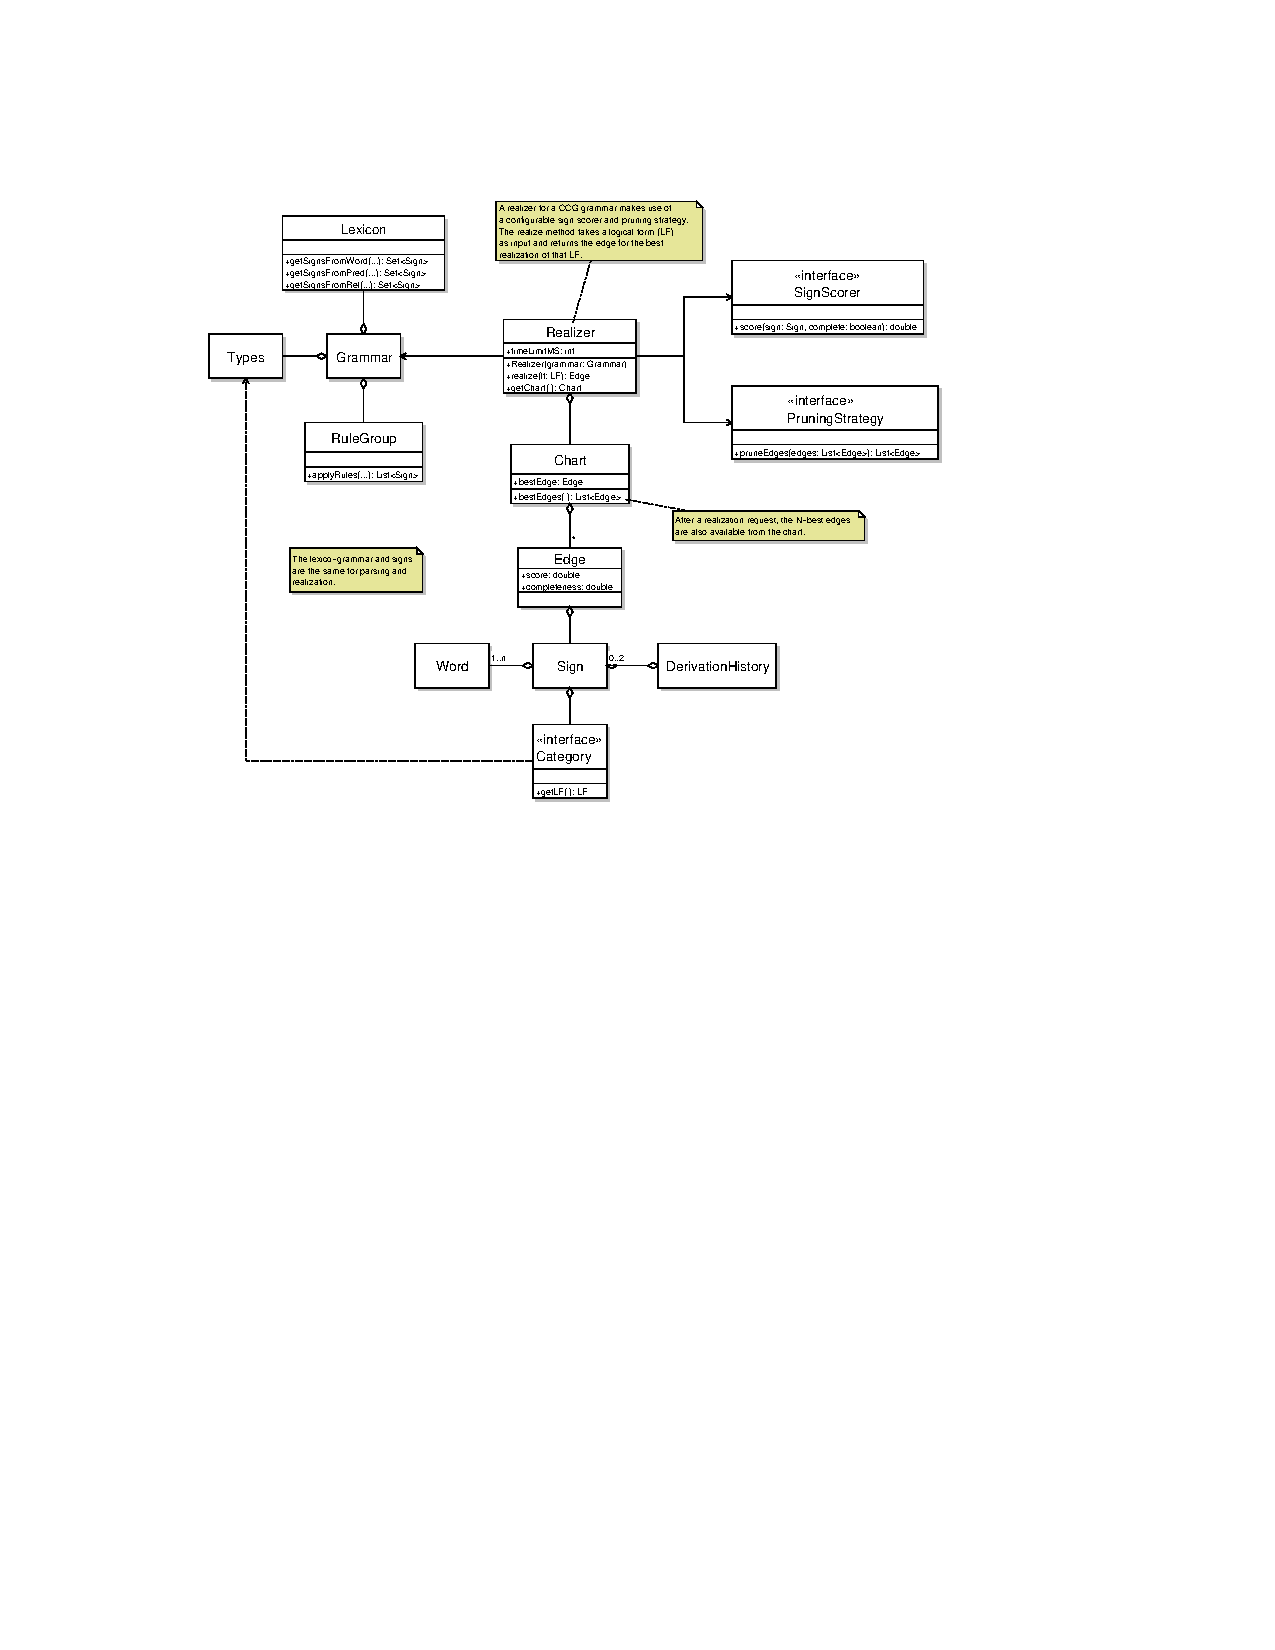
\includegraphics[width=\textwidth]{realizer-class.pdf} 
\caption{High-level architecture of the OpenCCG realizer}
\label{realizer-class}
\end{center}
\end{figure*}

The UML class diagram in Figure~\ref{realizer-class} shows the
high-level architecture of the OpenCCG realizer. A realizer
instance is constructed with a reference to a CCG grammar (which
supports both parsing and realization). The grammar's lexicon has
methods for looking up lexical items via their surface forms (for
parsing), or via the principal predicates or relations in their
semantics (for realization). A grammar also has a set of hierarchically
organized atomic types, which can serve as the values of features in the
syntactic categories, or as ontological sorts for the discourse
referents in the logical forms (LFs).

Lexical lookup yields lexical signs. A sign pairs a list of words with a
category, which itself pairs a syntactic category with a logical form.
Lexical signs are combined into derived signs using the rules in the
grammar's rule group. Derived signs maintain a derivation history, and
their word lists share structure with the word lists of their input
signs.

For generality, the realizer makes use of a configurable sign scorer and
pruning strategy. A sign scorer implements a function that returns a
number between 0 and 1 for an input sign. For example, a standard
trigram language model can be used to implement a sign scorer, by
returning the probability of a sign's words as its score. A pruning
strategy implements a method for determining which edges to prune during
the realizer's search. The input to the method is a ranked list of edges
for signs that have equivalent categories (but different words);
grouping edges in this way ensures that pruning cannot ``break'' the
realizer, i.e.\ prevent it from finding some grammatical derivation when
one exists. By default, an N-best pruning strategy is employed, which
keeps the N highest scoring input edges, pruning the rest (where N is
determined by the current preference settings).


\begin{figure*}%[p]%[t]%[!h]
\begin{center}
% \mbox{}
% \includegraphics{code/realize.pdf} 
\begin{lstlisting}
// load grammar, instantiate realizer
URL grammarURL = ...;
Grammar grammar = new Grammar(grammarURL);
Realizer realizer = new Realizer(grammar);

// configure realizer with trigram backoff model 
// and 10-best pruning strategy
realizer.signScorer = new StandardNgramModel(3, "lm.3bo");
realizer.pruningStrategy = new NBestPruningStrategy(10);

// ... then, for each request:

// get LF from input XML
Document inputDoc = ...;
LF lf = realizer.getLfFromDoc(inputDoc);

// realize LF and get output words in XML
Edge bestEdge = realizer.realize(lf);
Document outputDoc = bestEdge.sign.getWordsInXml();

// return output
... outputDoc ...;
\end{lstlisting}
\caption{Example realizer usage}
\label{realizer-usage}
\end{center}
\end{figure*}

\section{Using the realizer}

Sample Java code for using the realizer appears in
Figure~\ref{realizer-usage}. The input is an XML document that contains
an \code{lf} element either as the root or as a child of the root. To
create a sample XML document with an acceptable format, you can use the
\tccg\ tool's \code{:2xml <filename>} command. Note that the
input XML document can be created in any way that is allowed by the JDOM
API. For example, if the logical form is created by a Java XSLT-based
sentence planner in the same process, the XSLT output can be captured in
a JDOM document, and then simply passed by reference to the realizer.

The output of the realizer is typically an XML document, as shown in the
figure. In such documents, each word in the output sequence appears in
its own element; additionally, any pitch accents and boundary tones
appear in separate elements, and any expanded multi-words are indicated.
Output documents of this kind can be easily processed into other formats
using XSLT.  If a simple string output suffices, the
\code{Sign.getOrthography()} method can be used instead.

The realization algorithm is implemented by the \code{realize(LF)} method.
As in the chart realizers cited earlier, the algorithm makes use of a
chart and an agenda to perform a bottom-up dynamic programming search
for signs whose LFs completely cover the elementary predications in the
input logical form. The algorithm's details and a worked example appear
in \cite{White-RLAC:2004,White-INLG:2004}. To see a full realization
trace, you can use \ccgrz\ to realize an LF stored in an XML file (e.g.\
one created using \tccg). As shown in Figure~\ref{realizer-usage}, the
\code{realize(LF)} method returns the edge for the best realization of the
input LF, as determined by the sign scorer. After a realization request,
the N-best complete edges---or more generally, all the edges for
complete realizations that survived pruning---are also available from
the chart. To access these edges, you can invoke
\code{realizer.getChart().bestEdges()}.

The search for complete realizations proceeds in one of two modes,
anytime and two-stage (packing/unpacking). In the anytime mode, a
best-first search is performed with a configurable time limit (which may
be a limit on how long to look for a better realization, after the first
complete one is found). With this mode, the scores assigned by the sign
scorer determine the order of the edges on the agenda, and thus have an
impact on realization speed. In the two-stage mode, a packed forest of
all possible realizations is created in the first stage; then in the
second stage, the packed representation is unpacked in bottom-up
fashion, with scores assigned to the edge for each sign as it is
unpacked, much as in \cite{Langkilde:2000}. In both modes, the pruning
strategy is invoked to determine whether to keep or prune newly
constructed edges. For single-best output, the anytime mode can provide
signficant time savings by cutting off the search early; see
\cite{White-INLG:2004} for discussion. For N-best output---especially
when a complete search (up to the edges that survive the pruning
strategy) is desirable---the two-stage mode can be more efficient.


\section{Scoring signs}

The classes for implementing sign scorers appear in
Figure~\ref{scorer-class}. In the diagram, classes for n-gram scoring
appear towards the bottom, while classes for combining scorers appear on
the left, and the class for avoiding repetition appears on the right.

\begin{figure*}%[p]%[t]%[!h]
\begin{center}
\mbox{}
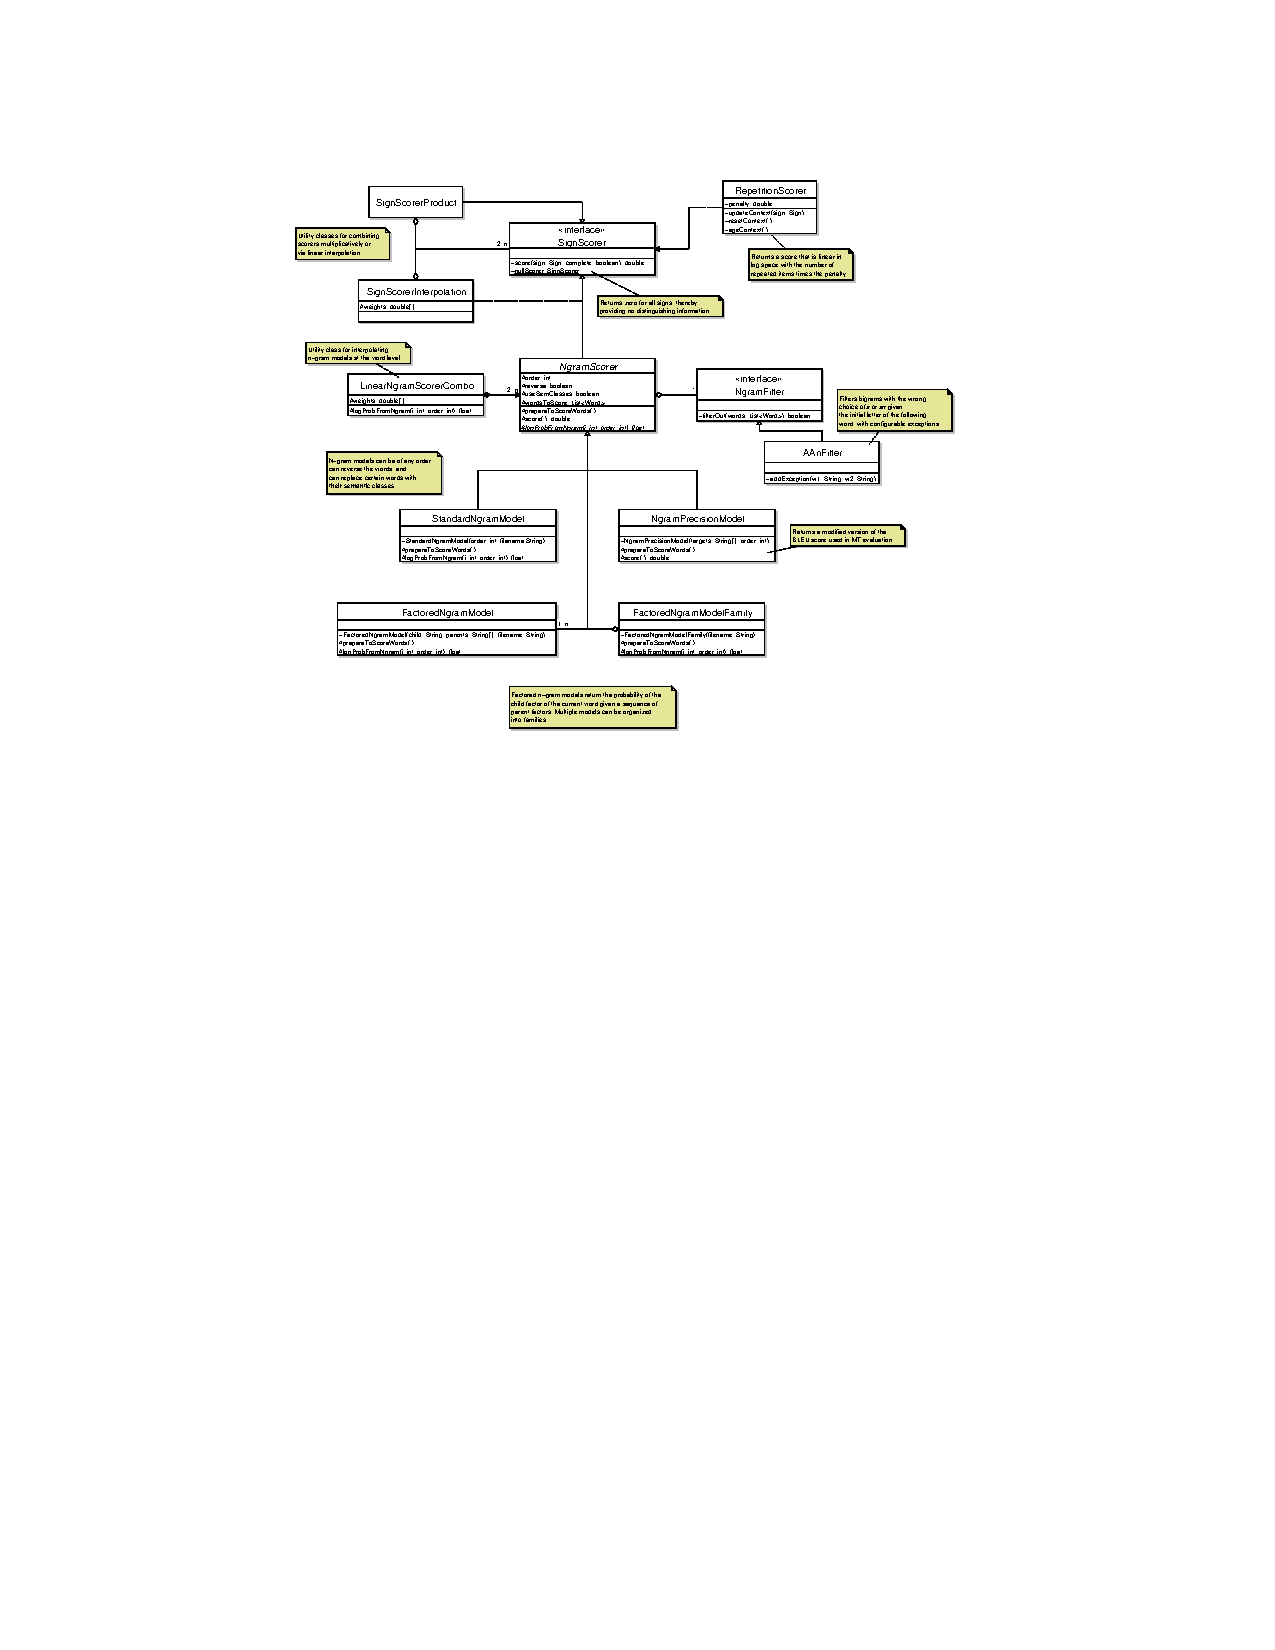
\includegraphics[width=\textwidth]{scorer-class.pdf} 
\caption{Classes for scoring signs}
\label{scorer-class}
\end{center}
\end{figure*}

\subsection{Standard n-gram models}
\label{standard-ngrams}

The \code{Standard\-Ngram\-Model} class can load standard n-gram backoff
models for scoring, as shown earlier in Figure~\ref{realizer-usage}.
Such models can be constructed with the SRILM toolkit
\cite{SRILM-ICSLP:2002}, as described in Section~\ref{using-srilm}; in
principle, other toolkits could be used instead, as long as their output
could be converted into the same file formats. Since the SRILM toolkit
has more restrictive licensing conditions than those of OpenCCG's LGPL
license, OpenCCG includes its own classes for scoring with n-gram
models, in order to avoid any necessary runtime dependencies on the
SRILM toolkit.

The n-gram tables are efficiently stored in a trie data structure (as in
the SRILM toolkit), thereby avoiding any arbitrary limit on the n-gram
order. To save memory and speed up equality tests, each string is
interned (replaced with a canonical instance) at load time, which
accomplishes the same purpose as replacing the strings with integers,
but without the need to maintain a separate mapping from integers back
to strings. For better generalization, certain words may be dynamically
replaced with the names of their semantic classes when looking up n-gram
probabilities. Words are assigned to semantic classes in the lexicon,
and the semantic classes to use in this way may be configured at the
grammar level. Note that \cite{Oh/Rudnicky:2002} and \cite{Adwait:2002}
make similar use of semantic classes in n-gram scoring, by deferring the
instantiation of classes (such as \textit{departure city}) until the end
of the generation process; our approach accomplishes the same goal in a
slightly more flexible way, in that it also allows the specific word to
be examined by other scoring models, if desired.

As discussed in \cite{White-INLG:2004}, with dialogue systems like COMIC
n-gram models can do an excellent job of placing underconstrained
adjectival and adverbial modifiers---as well as boundary tones---without
resorting to the more complex methods investigated for adjective
ordering in \cite{Shaw/Hatzi:1999,Malouf:2000}. For instance, in
examples like those in \eref{adv-placement}, they correctly select the
preferred positions for \textit{here} and \textit{also} (as well as for
the boundary tones), with respect to the verbal head and sister
dependents:
 
\begin{exe}
  %\small
  \ex \label{ex:adv-placement}
  \begin{xlist}
  \ex 
  Here$_{L+H*}$ LH\% we have a design in the classic$_{H*}$ style LL\% .
  \ex 
  This$_{L+H*}$ design LH\% here$_{L+H*}$ LH\% is also$_{H*}$ classic LL\% .
  \end{xlist}
\end{exe}

We have also found that it can be useful to use reverse (or
``right-to-left'') models, as they can help to place adverbs like
\textit{though}, as in \eref{though}:

\begin{exe}
  %\small
  \ex \label{ex:though}
  The tiles are also$_{H*}$ from the Jazz$_{H*}$ series though LL\% .
\end{exe}

\noindent In principle, the forward and reverse probabilities should be
the same---as they are both derived via the chain rule from the same
joint probability of the words in the sequence---but we have found that
with sparse data the estimates can differ substantially. In particular,
since \textit{though} typically appears at the end of a variety of
clauses, its right context is much more predictable than its left
context, and thus reverse models yield more accurate estimates of its
likelihood of appearing clause-finally. 

\subsection{N-gram scorers}

The \code{Standard\-Ngram\-Model} class is implemented as a subclass of
the base class \code{Ngram\-Scorer}. All \code{Ngram\-Scorer} instances
may have any number of \code{Ngram\-Filter} instances, whose
\code{filter\-Out} methods are invoked prior to n-gram scoring; if any
of these methods return true, a score of zero is immediately returned.
The \code{AAn\-Filter} provides one concrete implementation of the
\code{Ngram\-Filter} interface, and returns true if it finds a bigram
consisting of \textit{a} followed by a vowel-inital word, or \textit{an}
followed by a consonant-initial word, subject to a configurable set of
exceptions that can be culled from bigram counts. We have found that
such n-gram filters can be more efficient, and more reliable, than
relying on n-gram scores alone; in particular, with \textit{a/an}, since
the unigram probability for \textit{a} tends to be much higher than that
of \textit{an}, with unseen words beginning with a vowel, there may not
be a clear preference for the bigram beginning with \textit{an}.

The base class \code{Ngram\-Scorer} implements the bulk of the
\code{score} method, using an abstract \code{log\-Prob\-From\-Ngram} method
for subclass-specific calculation of the log probabilities (with
backoff) for individual n-grams. The \code{score} method also invokes
the \code{prepare\-To\-Score\-Words} method, in order to allow for
subclass-specific pre-processing of the words in the given sign. With
\code{Standard\-Ngram\-Model}, this method is used to extract the word forms
or semantic classes into a list of strings to score. It also appends any
pitch accents to the word forms or semantic classes, effectively
treating them as integral parts of the words.

Since the realizer builds up partial realizations bottom-up rather than
left-to-right, it only adds start of sentence (and end of sentence) tags
with complete realizations. As a consequence, the words with less than a
full $n-1$ words of history are scored with appropriate sub-models. For
example, the first word of a phrase is scored with a unigram sub-model,
without imposing backoff penalties.

Another consequence of bottom-up realization is that both the left- and
right-contexts may change when forming new signs from a given input
sign. Consequently, it is often not possible (even in principle) to use
the score of an input sign directly in computing the score of a new
result sign. If one could make assumptions about how the score of an
input sign has been computed---e.g., by a bigram model---one could
determine the score of the result sign from the scores of the input
signs together with an adjustment for the word(s) whose context has
changed. However, our general approach to sign scoring precludes making
such assumptions. Nevertheless, it is still possible to improve the
efficiency of n-gram scoring by caching the log probability of a sign's
words, and then looking up that log probability when the sign is used as
the first input sign in creating a new combined sign---thus retaining
the same left context---and only recomputing the log probabilities for
the words of any input signs past the first one. (With reverse models,
the sign must be the last sign in the combination.) In principle, the
derivation history could be consulted further to narrow down the words
whose n-gram probabilities must be recomputed to the minimum possible,
though \code{Ngram\-Scorer} only implements a single-step lookup at
present.\footnote{Informal experiments indicate that caching log
probabilities in this way can yield an overall reduction in best-first
realization times of 2-3\% on average.} Finally, note that a Java
\code{Weak\-Hash\-Map} is used to implement the cache, in order to avoid
an undesirable buildup of entries across realization requests.

\subsection{Interpolation}
\label{interpolation}

Scoring models may be linearly interpolated in two ways.  Sign scorers
of any variety may be combined using the \code{Sign\-Scorer\-Interpolation} 
class.  For example, Figure~\ref{forward-reverse-interpolation} shows 
how forward and reverse n-gram models may be interpolated.

\begin{figure*}%[p]%[t]%[!h]
\begin{center}
\begin{lstlisting}
// configure realizer with 4-gram forward and reverse backoff 
// models, interpolated with equal weight
NgramScorer forwardModel = new StandardNgramModel(4, "lm.4bo"); 
NgramScorer reverseModel = new StandardNgramModel(4, "lm-r.4bo"); 
reverseModel.setReverse(true);
realizer.signScorer = new SignScorerInterpolation(
    new SignScorer[] { forwardModel, reverseModel }
);
\end{lstlisting}
\caption{Example interpolated n-gram model}
\label{forward-reverse-interpolation}
\end{center}
\end{figure*}

With n-gram models of the same direction, it is also possible to
linearly interpolate models at the word level, using the
\code{Linear\-Ngram\-Scorer\-Combo} class. Word-level interpolation
makes it easier to use cache models created with maximum likelihood
estimation, as word-level interpolation with a base model avoids
problems with zero probabilities in the cache model. As discussed in
\cite{Carsten-Alignment:2005}, cache models can be used to promote
alignment with a conversational partner, by constructing a cache model
from the bigrams in the partner's previous turn, and interpolating it
with a base model.\footnote{At present, such cache models must be
constructed with a call to the SRILM toolkit; it would not be difficult
to add OpenCCG support for constructing them though, since these models
do not require smoothing.} Figure~\ref{base-cache-interpolation} shows
one way to create such an interpolated model.

\begin{figure*}%[p]%[t]%[!h]
\begin{center}
\begin{lstlisting}
// configure realizer with 4-gram backoff base model, 
// interpolated at the word level with a bigram maximum-likelihood 
// cache model, with more weight given to the base model
NgramScorer baseModel = new StandardNgramModel(4, "lm.4bo"); 
NgramScorer cacheModel = new StandardNgramModel(2, "lm-cache.mle"); 
realizer.signScorer = new LinearNgramScorerCombo(
    new SignScorer[] { baseModel, cacheModel }, 
    new double[] { 0.6, 0.4 }
);
\end{lstlisting}
\caption{Example word-level interpolation of a cache model}
\label{base-cache-interpolation}
\end{center}
\end{figure*}

\subsection{N-gram precision models}
\label{ngram-precision}

The \code{NgramPrecisionModel} subclass of \code{Ngram\-Scorer} computes a
modified version of the Bleu score used in MT evaluation
\cite{Bleu:2001}. Its constructor takes as input an array of target
strings---from which it extracts the n-gram sequences to use in
computing the n-gram precision score---and the desired order. Unlike
with the Bleu score, rank order centroid weights (rather than the
geometric mean) are used to combine scores of different orders, which
avoids problems with scoring partial realizations which have no n-gram
matches of the target order. For simplicity, the score also does not
include the Bleu score's bells and whistles to make cheating on length
difficult.
 
We have found n-gram precision models to be very useful for regression
testing the grammar, as an n-gram precision model created just from the
target string nearly always leads the realizer to choose that exact
string as its preferred realization. These models can also be useful for
evaluating the success of different scoring models in a cross-validation
setup, though with high quality output, manual inspection is usually
necessary to determine the importance of any differences between the
preferred realization and the target string. Finally, note that n-gram
precision models can be used as a quick-and-dirty substitute for
standard n-gram models, if one does not have time to install and use the
SRILM toolkit.

\subsection{Factored language models}

A factored language model \cite{Bilmes-Kirchoff:2003} is a new kind of
language model that treats words as bundles of factors. To support
scoring with such models, OpenCCG represents words as objects with a
surface form, pitch accent, stem, part of speech, supertag, and semantic
class. Words may also have any number of further attributes, such as
associated gesture classes, in order to handle in a general way elements
like pitch accents that are ``coarticulated'' with words. 

To represent words efficiently, and to speed up equality tests, all
attribute values are interned, and the \code{Word} objects themselves
are interned via a factory method. Note that in Java, it is
straightforward to intern objects other than strings by employing a
\code{Weak\-Hash\-Map} to map from an object key to a weak reference to
itself as the canonical instance. (Using a weak reference avoids
accumulating interned objects that would otherwise be garbage
collected.)

With the SRILM toolkit, factored language models can be constructed that
support \textit{generalized parallel backoff}: that is, backoff order is
not restricted to just dropping the most temporally distant word first,
but rather may be specified as a path through the set of contextual
parent variables; additionally, parallel backoff paths may be specified,
with the possibility of combining these paths dynamically in various
ways. In OpenCCG, the \code{Factored\-Ngram\-Model} class supports
scoring with factored language models that employ generalized backoff,
though parallel backoff is not yet supported, as it remains somewhat
unclear whether the added complexity of parallel backoff is worth the
implementation effort. Typically, several related factored language
models are specified in a single file and loaded by a
\code{Factored\-Ngram\-Model\-Family}, which can multiplicatively score
models for different child variables, and include different sub-models
for the same child variable.

To illustrate, let us consider a simplified version of the factored
language model family used in the COMIC realizer. This model computes
the probability of the current word given the preceding ones according
to the formula shown in \eref{comic-flm}, where a word consists of the
factors word (W), pitch accent (A), gesture class (GC), and gesture
instance (GI), plus the other standard factors which the model ignores:

\begin{exe}
\ex \label{ex:comic-flm}
\begin{small}
\(
\begin{array}{l}
P(\langle W,A,GC,GI \rangle \, | \, \langle W,A,GC,GI \rangle_{-1} \, \ldots) \approx  \\
\; \; \; P(W \, | \, W_{-1} W_{-2} A_{-1} A_{-2}) \; \times \\
\; \; \; P(GC \, | \, W) \; \times \\
\; \; \; P(GI \, | \, GC) \\
\end{array}
\)
\end{small}
\end{exe}

\noindent In \eref{comic-flm}, the probability of the current word is
approximated by the probability of the current word form given the
preceding two word forms and preceding two pitch accents, multiplied by
the probability of the current gesture class given the current word
form, and by the probability of the current gesture instance given the
current gesture class. Note that in the COMIC grammar, the choice of
pitch accent is entirely rule governed, so the current pitch accent is
not scored separately in the model. However, the preceding pitch accents
are taken into account in predicting the current word form, as
perplexity experiments have suggested that they do provide additional
information beyond that provided by the previous word forms.

The specification file for this model appears in Figure~\ref{flm-spec}.
The format of the file is a restricted form of the files used by the
SRILM toolkit to build factored language models. The file specifies four
models, where the first, third and fourth models correspond to those in
\eref{comic-flm}. With the first model, since the previous words are
typically more informative than the previous pitch accents, the backoff
order specifies that the most distant accent, \code{A(-2)}, should be
dropped first, followed by the previous accent, \code{A(-1)}, then the
most distant word, \code{W(-2)}, and finally the previous word,
\code{W(-1)}. The second model is considered a sub-model of the
first---since it likewise predicts the current word---to be used when
there is only one word of context available (i.e.\ with bigrams). Note
that when scoring a bigram, the second model will take the previous
pitch accent into account, whereas the first model would not. For
documentation of the file format as it is used in the SRILM toolkit, see
\cite{FLM-JHSW:2002}.

\begin{figure*}%[p]%[t]%[!h]
\begin{footnotesize}
\begin{verbatim}
## Simplified COMIC realizer FLM spec file

## Trigram Word model based on previous words and accents, dropping accents first, 
##   with bigram sub-model;
## Unigram Gesture Class model based on current word; and 
## Unigram Gesture Instance model based on current gesture class

4

## 3gram with A
W : 4 W(-1) W(-2) A(-1) A(-2) w_w1w2a1a2.count w_w1w2a1a2.lm 5
  W1,W2,A1,A2  A2 ndiscount gtmin 1 
  W1,W2,A1  A1 ndiscount gtmin 1 
  W1,W2  W2 ndiscount gtmin 1 
  W1  W1 ndiscount gtmin 1 
  0   0  ndiscount gtmin 1

## bigram with A
W : 2 W(-1) A(-1) w_w1a1.count w_w1a1.lm 3
  W1,A1  A1  ndiscount gtmin 1 
  W1  W1  ndiscount gtmin 1 
  0   0   ndiscount gtmin 1

## Gesture class depends on current word
GC : 1 W(0) gc_w0.count gc_w0.lm 2
  W0  W0 ndiscount gtmin 1 
  0   0  ndiscount gtmin 1

## Gesture instance depends only on class
GI : 1 GC(0) gi_gc0.count gi_gc0.lm 2
  GC0  GC0 ndiscount gtmin 1
  0 0
\end{verbatim}
\end{footnotesize}
\caption{Example factored language model family specification}
\label{flm-spec}
\end{figure*}

Like \code{Standard\-Ngram\-Model}, the \code{Factored\-Ngram\-Model} class
stores its n-gram tables in a trie data structure, except that it stores
an interned factor key (i.e.\ a factor name and value pair, or just a
string, in the case of the word form) at each node, rather than a simple
string. During scoring, the \code{log\-Prob\-From\-Ngram} method determines
the log probability (with backoff) of a given n-gram by extracting the
appropriate sequence of factor keys, and using them to compute the log
probability as with standard n-gram models. The
\code{Factored\-Ngram\-Model\-Family} class computes log probabilities by
delegating to its component factored n-gram models (choosing appropriate
sub-models, when appropriate) and summing the results.
 
\subsection{Avoiding repetition}

While cache models appear to be a promising avenue to promote lexical
and syntactic alignment with a conversational partner, a different
mechanism appears to be called for to avoid ``self-alignment''---that
is, to avoid the repetitive use of words and phrases. As a means to
experiment with avoiding repetition, OpenCCG includes the
\code{Repetition\-Scorer} class. This class makes use of a configurable
penalty plus a set of methods for dynamically managing the context. It
returns a score of \( 10^{- c_r \times p} \), where $c_r$ is the count
of repeated items, and $p$ is the penalty. Note that this formula
returns 1 if there are no repeated items, and returns a score that is
linear in log space with the number of repeated items otherwise.

A repetition scorer can be combined multiplicatively with an n-gram
model, in order to discount realizations that repeat items from the
recent context. Figure~\ref{rep-scorer} shows such a combination,
together with the operations for updating the context. By default, open
class stems are the considered the relevant items over which to count
repetitions, though this behavior can be specialized by subclassing
\code{Repetition\-Scorer} and overriding the \code{updateItems} method.
Note that in counting repetitions, full counts are given to items in the
previous words or recent context, while fractional counts are given to
older items; the exact details may likewise be changed in a subclass, by
overriding the \code{repeatedItems} method.

\begin{figure*}%[p]%[t]%[!h]
\begin{center}
\begin{lstlisting}
// set up n-gram scorer and repetition scorer
String lmfile = "ngrams/combined.flm";
NgramScorer ngramScorer = new FactoredNgramModelFamily(lmfile, true);
ngramScorer.addFilter(new AAnFilter());
RepetitionScorer repetitionScorer = new RepetitionScorer();

// combine n-gram scorer with repetition scorer
realizer.signScorer = new SignScorerProduct(
    new SignScorer[] { ngramScorer, repetitionScorer }
);

// ... then, after each realization request, 
Edge bestEdge = realizer.realize(lf);

// ... update repetition context for next realization:
repetitionScorer.ageContext();
repetitionScorer.updateContext(bestEdge.getSign());
\end{lstlisting}
\caption{Example combination of an n-gram scorer and a repetition scorer}
\label{rep-scorer}
\end{center}
\end{figure*}

\subsection{Building language models with the SRILM toolkit}
\label{using-srilm}

You can use \occg's regression testing tool, \ccgtest, to help build and
test language models built with the SRILM toolkit. By default, running
\ccgtest\ will use the grammar in the current directory to parse and
realize the default regression file, \code{testbed.xml}, using an n-gram
precision model constructed for each test item. Using the appropriate
command-line options, it is also possible to export the text of the test
items in order to construct an n-gram model with the SRILM toolkit, and
then use the resulting model in testing the realizer.

To display the syntax of \ccgtest's command-line options, you can invoke
it with the the \code{-h} option, as shown in \eref{ccg-test-help}. To
export the text of the test items to a text file, you use the
\code{-text} option, as in \eref{export-text}. The next step is to use
SRILM's \code{ngram-count} tool to build an n-gram language model. In
\eref{make-lm},\footnote{This command, and the ensuing ones, should be
entered on one line.} \code{ngram-count} is used to build a 4-gram
backoff model, \code{n.4bo}, from the text file \code{tb.txt}, using
Ristad's ``natural'' discounting method \cite{Ristad:1995}. For small
test sets, we have found that Ristad's method works better than the
default one (Good-Turing). Note that in \eref{make-lm}, the \code{-unk}
option is used to reserve some probability for unknown words; the
\code{-gt<N>min 1} options (for N=1 to 4) specify to keep all 1-counts;
and the \code{-ndiscount<N>} options (for N=1 to 4) specify the use of
natural discounting for unigrams through 4-grams. Finally, to test the
resulting language model, you use \ccgtest's \code{-ngramorder} and
\code{-lm} options, as shown in \eref{test-lm}.

\begin{exe}
  %\small
  \ex %\label{ex:make-test-lm}
  \begin{xlist}
  \ex \label{ex:ccg-test-help}
  \code{ccg-test -h}
  \ex \label{ex:export-text} 
  \code{ccg-test -text tb.txt}
  \ex \label{ex:make-lm} 
  \code{ngram-count -order 4 -unk -text tb.txt -lm n.4bo \\
  -gt1min 1 -gt2min 1 -gt3min 1 -gt4min 1 \\
  -ndiscount1 -ndiscount2 -ndiscount3 -ndiscount4}
  \ex \label{ex:test-lm}
  \code{ccg-test -noparsing -ngramorder 4 -lm n.4bo}
  \end{xlist}
\end{exe}

To perform a simple 2-fold cross-validation, \ccgtest\ includes options
for exporting or testing just the even or odd test items. The command in
\eref{export-even} shows how you can export just the text of the
even-numbered test items. Note that the \code{-textsc} option specifies
that the text be exported using semantic class replacement, i.e.\ with
certain words replaced with their semantic classes; the classes to use
for this purpose are specified using the \code{replacement-sem-classes}
attribute of the \code{tokenizer} element in the \code{grammar.xml}
file.  The next step is to build a language model just as before; the
abbreviated command appears in \eref{make-even-lmsc}.  Finally, you can
test the language model on just the odd-numbered items, as in
\eref{test-odd}, where the \code{-lmsc} option specifies that semantic
class replacement should be employed when scoring realizations with the
model.  Naturally, you can switch the \code{-even} and \code{-odd}
flags, and adjust the text and language model names, to test realization
on the even-numbered items, using a language model trained from the
odd-numbered ones.

\begin{exe}
  %\small
  \ex %\label{ex:even-odd}
  \begin{xlist}
  \ex \label{ex:export-even} 
  \code{ccg-test -even -textsc tb-sc.even.txt}
  \ex \label{ex:make-even-lmsc} 
  \code{ngram-count -order 4 -unk -text tb-sc.even.txt \\
  -lm n-sc.even.4bo ...}
  \ex \label{ex:test-odd}
  \code{ccg-test -noparsing -odd -ngramorder 4 -lmsc n-sc.even.4bo}
  \end{xlist}
\end{exe}

An example of building a factored language model appears next. In
\eref{export-fsc}, the text of the test items is exported, where each
word appears with all its factors, and word forms are replaced with
semantic classes when appropriate.  In \eref{make-flmsc}, SRILM's
\code{fngram-count} is used to create a factored language model from the
spec file named \code{spec.flm}.  (Note that the various individual
language model files are listed in the spec file.)  Finally,
\eref{test-flm} shows how the factored language model can be tested in
\ccgtest.

\begin{exe}
  %\small
  \ex 
  \begin{xlist}
  \ex \label{ex:export-fsc} 
  \code{ccg-test -textfsc tb-fsc.txt}
  \ex \label{ex:make-flmsc} 
  \code{fngram-count -factor-file spec.flm -text tb-fsc.txt -lm -unk}
  \ex \label{ex:test-flm}
  \code{ccg-test -noparsing -flmsc spec.flm}
  \end{xlist}
\end{exe}


\section{Pruning Strategies}
\label{pruning}

The classes for defining edge pruning strategies appear in
Figure~\ref{pruner-class}. As mentioned in Section~\ref{overview}, an N-best
pruning strategy is employed by default, where N is determined by the
current preference settings. It is also possible to define custom
strategies. To support the definition of a certain kind of custom
strategy, the abstract class \code{Diversity\-Pruning\-Strategy}
provides an N-best pruning strategy that promotes diversity in the edges
that are kept, according to the equivalence relation established by the
abstract \code{not\-Compellingly\-Different} method. In particular, in
order to determine which edges to keep, a diversity pruning strategy
clusters the edges into a ranked list of equivalence classes, which are
sequentially sampled until the limit N is reached. If the
\code{single\-Best\-Per\-Group} flag is set, then a maximum of one edge
per equivalence class is retained.

\begin{figure*}%[p]%[t]%[!h]
\begin{center}
\mbox{}
%scale=1.25
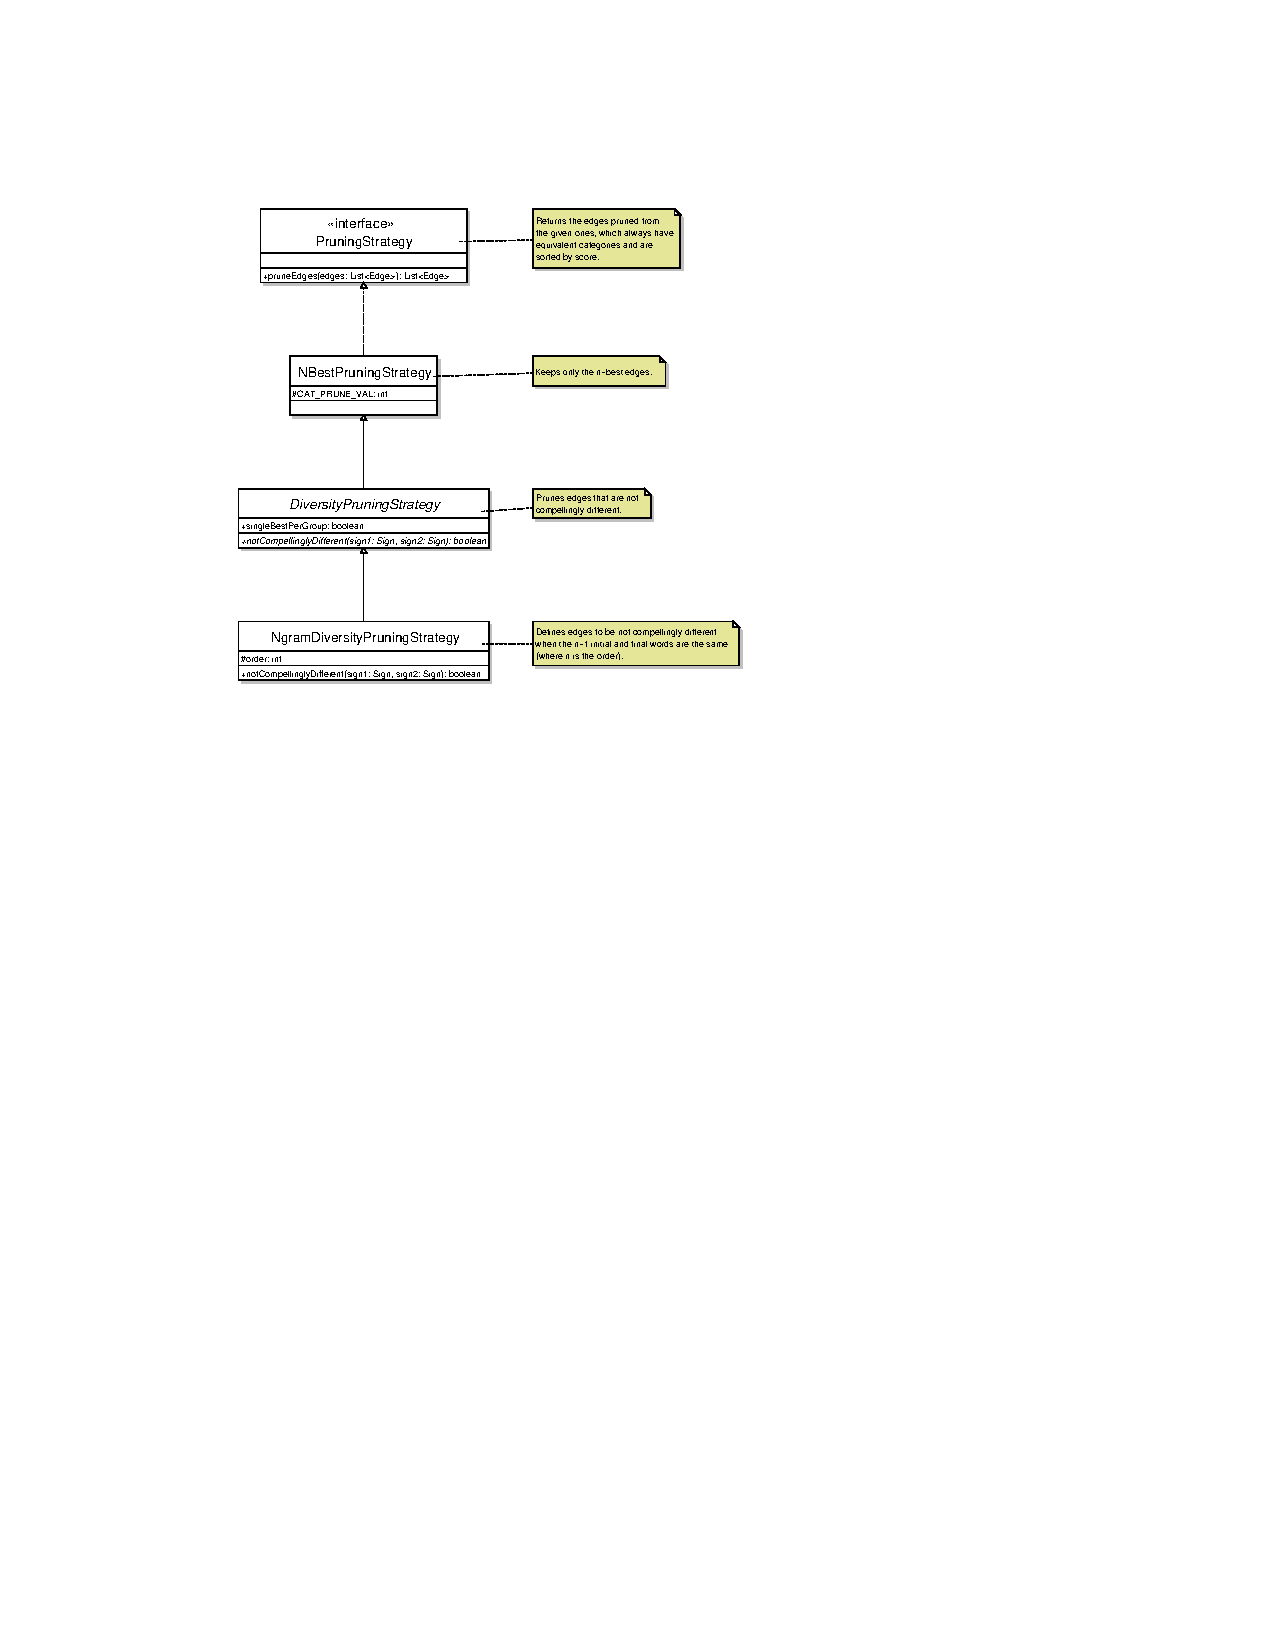
\includegraphics[width=\textwidth]{pruner-class.pdf} 
\caption{Classes for defining pruning strategies}
\label{pruner-class}
\end{center}
\end{figure*}

As an example, the COMIC realizer's diversity pruning strategy appears
in Figure~\ref{gest-diversity-strategy}. The idea behind this strategy
is to avoid having the N-best lists become full of signs whose words
differ only in the exact gesture instance associated with one or more of
the words. With this strategy, if two signs differ in just this way, the
edge for the lower-scoring sign will be considered ``not compellingly
different'' and pruned from the N-best list, making way for other edges
whose signs exhibit more interesting differences.

\begin{figure*}%[p]%[t]%[!h]
\begin{center}
\begin{lstlisting}
// configure realizer with gesture diversity pruner
realizer.pruningStrategy = new DiversityPruningStrategy() {
  /** 
   * Returns true iff the given signs are not compellingly different; 
   * in particular, returns true iff the words differ only in their  
   * gesture instances. */
  public boolean notCompellinglyDifferent(Sign sign1, Sign sign2) {
    List words1 = sign1.getWords(); List words2 = sign2.getWords();
    if (words1.size() != words2.size()) return false;
    for (int i = 0; i < words1.size(); i++) {
      Word w1 = (Word) words1.get(i); Word w2 = (Word) words2.get(i);
      if (w1 == w2) continue;
      if (w1.getForm() != w2.getForm()) return false;
      if (w1.getPitchAccent() != w2.getPitchAccent()) return false;
      if (w1.getVal("GC") != w2.getVal("GC")) return false;
      // nb: assuming that they differ in the val of GI at this point 
    }
    return true;
  }
};
\end{lstlisting}
\caption{Example diversity pruning strategy}
\label{gest-diversity-strategy}
\end{center}
\end{figure*}

OpenCCG also provides a concrete subclass of
\code{Diversity\-Pruning\-Strategy} named
\code{Ngram\-Diversity\-Pruning\-Strategy}, which generalizes the
approach to pruning described in \cite{Langkilde:2000}. With this class,
two signs are considered not compellingly different if they share the
same $n\!-\!1$ initial and final words, where $n$ is the n-gram order.
When one is interested in single-best output, an n-gram diversity
pruning strategy can increase efficiency while guaranteeing no loss in
quality---as long as the reduction in the search space outweighs the
extra time necessary to check for the same initial and final
words---since any words in between an input sign's $n\!-\!1$ initial and
final ones cannot affect the n-gram score of a new sign formed from the
input sign. However, when N-best outputs are desired, or when repetition
scoring is employed, it is less clear whether it makes sense to use an
n-gram diversity pruning strategy; for this reason, a simple N-best
strategy remains the default option.


\section{Disjunctive logical forms}
\label{sec:disj-lf}

In applications, to specify the desired space of possible paraphrases,
one may either provide an input logical form that underspecifies certain
realization choices, or include explicit disjunctions in the input LF
(or both). In our experience, we have found disjunctive LFs---inspired
by those found in \cite{Shemtov:PhD}---to be an important capability,
especially as one seeks to make grammars reusable across applications.

\begin{figure}%[t]%[!h]
\begin{small}
\begin{center}
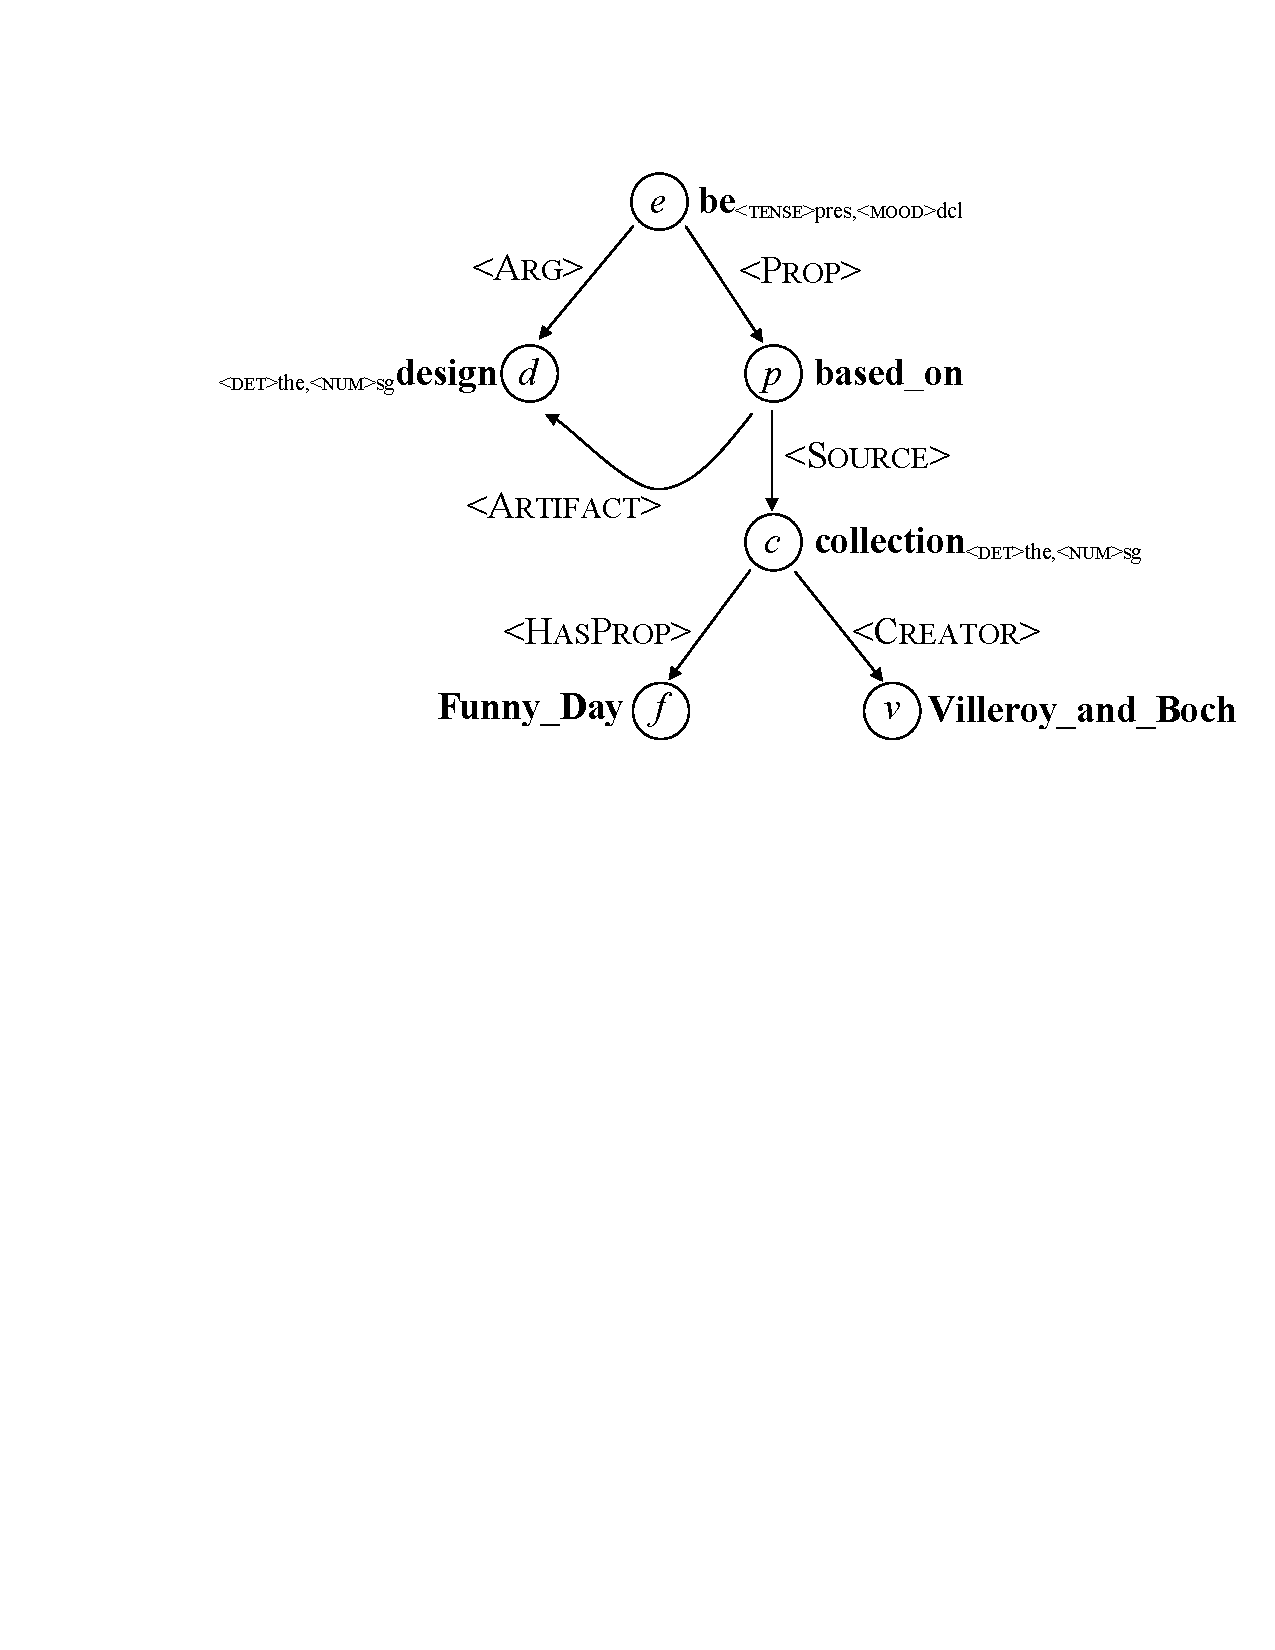
\includegraphics[width=0.52\textwidth]{ex1a} 
\end{center}
\begin{itemize}
\item[(a)] Semantic dependency graph for \textit{The design (is$\mid$'s) 
based on the Funny Day collection by Villeroy and Boch.}
\end{itemize}

\vspace{3mm}
\begin{center}
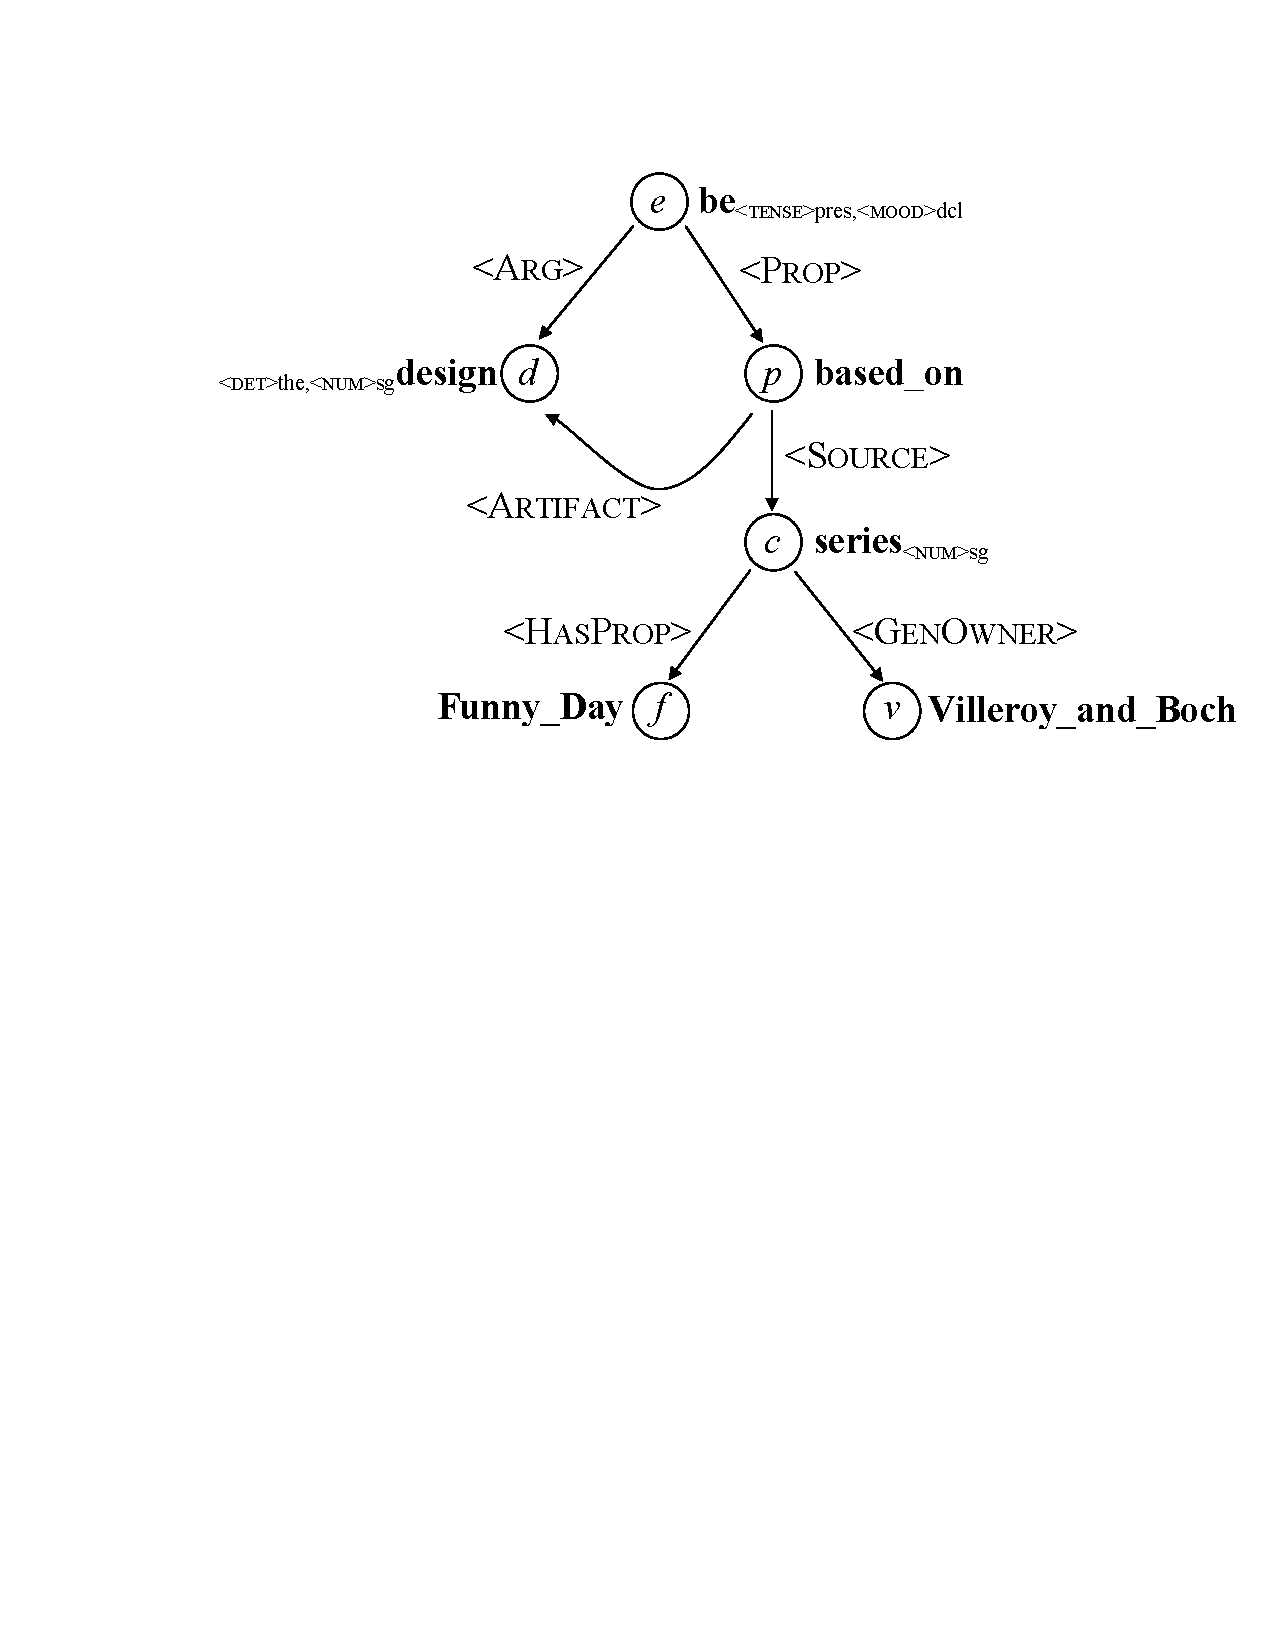
\includegraphics[width=0.52\textwidth]{ex1b} 
\end{center}
\begin{itemize}
\item[(b)] Semantic dependency graph for \textit{The design (is$\mid$'s) 
based on Villeroy and Boch's Funny Day series.}
\end{itemize}

\vspace{3mm}
\begin{center}
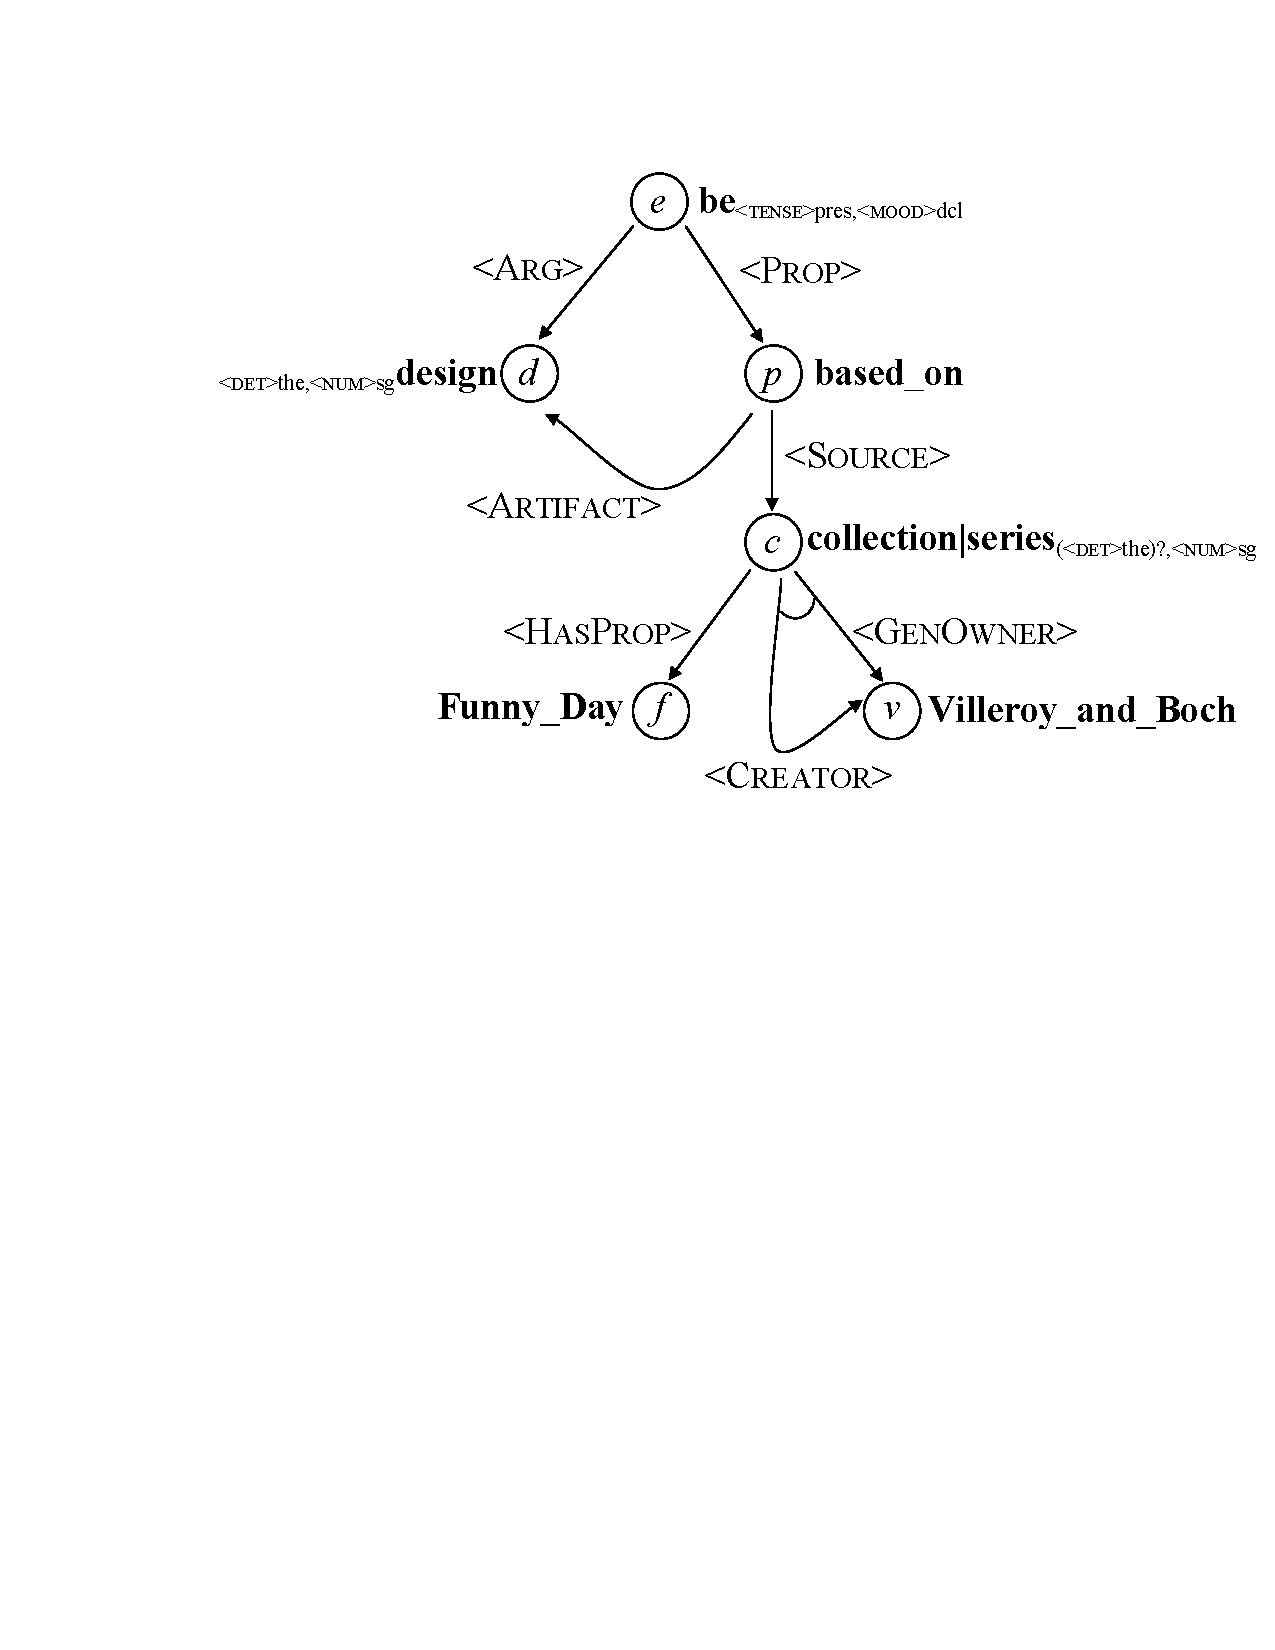
\includegraphics[width=0.52\textwidth]{ex1c} 
\end{center}
\begin{itemize}
\item[(c)] Disjunctive semantic dependency graph covering (a)-(b), i.e.\
\textit{The design (is$\mid$'s) based on 
(the Funny Day (collection$\mid$series) by Villeroy and Boch $\mid$
Villeroy and Boch's Funny Day (collection$\mid$series)).}
\end{itemize}
\end{small}

\caption{Example semantic dependency graphs.}
\label{fig:ex1}
\end{figure}

\begin{figure}%[t]%[!h]
\begin{small}
\ensuremath{
@_{e}(\C{be} \wedge \modp{tense}\con{pres} \wedge \modp{mood}\con{dcl} \wedge \\
    \mytab{@_{e}(}
    \modp{Arg}(d \wedge \C{design} \wedge \modp{det}\con{the} \wedge \modp{num}\con{sg}) \wedge \\
    \mytab{@_{e}(}
    \modp{Prop}(p \wedge \C{based-on} \wedge \\
                \mytab{@_{e}(\modp{Prop}(}
                \modp{Artifact}d \wedge \\
                \mytab{@_{e}(\modp{Prop}(}
                \modp{Source}(c \wedge \C{collection} \wedge \modp{det}\con{the} \wedge \modp{num}\con{sg} \wedge \\
                              \mytab{@_{e}(\modp{Prop}(\modp{Source}(}
                              \modp{HasProp}(f \wedge \C{Funny\_Day}) \wedge \\
                              \mytab{@_{e}(\modp{Prop}(\modp{Source}(}
                              \modp{Creator}(v \wedge \C{V\&B}))))
}

\begin{center}
(a)

\vspace{2mm}
\mbox{}\vdots
\vspace{2mm}
\end{center}

\ensuremath{
@_{e}(\C{be} \wedge \modp{tense}\con{pres} \wedge \modp{mood}\con{dcl} \wedge \\
    \mytab{@_{e}(}
    \modp{Arg}(d \wedge \C{design} \wedge \modp{det}\con{the} \wedge \modp{num}\con{sg}) \wedge \\
    \mytab{@_{e}(}
    \modp{Prop}(p \wedge \C{based-on} \wedge \\
                \mytab{@_{e}(\modp{Prop}(}
                \modp{Artifact}d \wedge \\
                \mytab{@_{e}(\modp{Prop}(}
                \modp{Source}(c \wedge \modp{num}\con{sg} \wedge (\modp{det}\con{the})? \wedge \\
                              \mytab{@_{e}(\modp{Prop}(\modp{Source}(}
                              (\C{collection} \xor \C{series}) \wedge \\
                              \mytab{@_{e}(\modp{Prop}(\modp{Source}(}
                              \modp{HasProp}(f \wedge \C{Funny\_Day}) \wedge \\
                              \mytab{@_{e}(\modp{Prop}(\modp{Source}(}
                              (\modp{Creator}\shared{v} \xor \modp{GenOwner}\shared{v})))) \\
\wedge @_{v}(\C{Villeroy\_and\_Boch})
}

\begin{center}
(c)
\end{center}
\end{small}

\caption{HLDS for examples in \figref{ex1}.}
\label{fig:ex1-hlds}
\end{figure}

As an illustration of disjunctive logical forms, consider the semantic
dependency graphs in \figref{ex1}, which are taken from the
COMIC\footnote{\texttt{http://www.hcrc.ed.ac.uk/comic/}} multimodal
dialogue system.\footnote{To simplify the exposition, the features
  specifying information structure and deictic gestures have been
  omitted, as have the semantic sorts of the discourse referents.}
Given the lexical categories in the COMIC grammar, the graphs in
\figref{ex1}(a) and (b) fully specify their respective realizations,
with the exception of the choice of the full or contracted form of the
copula.\footnote{Note that to be consistent with the distributed
  grammar, the predicate $\C{based\_on}$ should actually be
  $\C{based-on}$; this discrepancy has been corrected in the
  subsequent figures.} To generalize over these alternatives, the
disjunctive graph in (c) may be employed.  This graph allows a free
choice between the domain synonyms \textit{collection} and
\textit{series}, as indicated by the vertical bar between their
respective predications. The graph also allows a free choice between
the \modp{Creator} and \modp{GenOwner} relations---lexicalized via
\textit{by} and the possessive, respectively---connecting the head $c$
(\textit{collection} or \textit{series}) with the dependent $v$ (for
\textit{Villeroy and Boch}); this choice is indicated by an arc
between the two dependency relations.\footnote{Note that the arc and
  vertical bar are just presentation devices; there is no difference
  in the underlying implementation.} Finally, the determiner feature
(\modp{det}\con{the}) on $c$ is indicated as optional, via the
question mark.\footnote{Another option would be to include the
  determiner feature in the alternative with the \modp{Creator}
  relation, but that would make the graph harder to draw and would not
  illustrate optionality.}

It is worth pausing at this point to observe that in designing the
COMIC grammar, the differences between (a) and (b) could perhaps have
been collapsed.  However, such a move would make it more difficult to
reuse the grammar in other applications---and indeed, the core of the
grammar is shared with the FLIGHTS system
\cite{FLIGHTS-FLAIRS:2004}---as it would presuppose that these
paraphrases should always available in the same contexts.  An example
where the disjunctively specified paraphrases have applicable contexts
that are more clearly limited appears in \eref{ex2}:

\begin{exe}
\ex \label{ex:ex2}
(This design $\mid$ This one $\mid$ This) (is$\mid$'s) (classic $\mid$
in the classic style) $\mid$ Here we have a (classic design $\mid$
design in the classic style).
\end{exe}

\noindent This example shows some of the phrasings that may be used in
COMIC to describe the style of a design that has not been discussed
previously.  The example includes a top-level disjunction between the
use of a deictic NP \textit{this design $\mid$ this one $\mid$ this}
(with an accompanying pointing gesture) followed by the copula, or the
use of the phrase \textit{here we have} to introduce the design.
While these alternatives can function as paraphrases in this context,
it is difficult to see how one might specify them in a single
underspecified (and application-neutral) logical form.

Graphs such as those in \figref{ex1} are represented internally using
Hybrid Logic Dependency Semantics (HLDS), as in \figref{ex1-hlds}. In
HLDS, as can be seen in \figref{ex1-hlds}(a), each semantic head is
associated with a nominal that identifies its discourse referent, and
heads are connected to their dependents via dependency relations, which
are modeled as modal relations; modal relations are also used to
represent semantic features (in which case the relation is to an
anonymous node). In (c), two new operators are introduced to represent
periphrastic alternatives and optional parts of the meaning, namely
$\xor$ and $(\cdot)?$, for exclusive-or and optionality, respectively.
To indicate that a nominal represents a reference to a node that is
considered a shared part of multiple alternatives, the nominal is
annotated with a box, as exemplified by \shared{v}. This notion of
shared references is needed during the logical form flattening stage of
the realization algorithm in order to determine which elementary
predications are part of each alternative.

\begin{figure}%[t]%[!h]
\begin{footnotesize}
\begin{verbatim}
<node id="e" pred="be" tense="pres" mood="dcl">
  <rel name="Arg"> 
    <node id="d" pred="design" det="the" num="sg"/>
  </rel>
  <rel name="Prop">
    <node id="p" pred="based-on">
      <rel name="Artifact"> <node idref="d"/> </rel>
      <rel name="Source"> 
        <node id="c" pred="collection" det="the" num="sg">
          <rel name="HasProp"> 
            <node id="f" pred="Funny_Day"/>
          </rel>
          <rel name="Creator"> 
            <node id="v" pred="Villeroy_and_Boch"/>
          </rel> 
        </node>
      </rel>
    </node>
  </rel>
</node>
\end{verbatim}
\end{footnotesize}

\caption{XML for example (a) \figref{ex1}.}
\label{fig:ex1-xml-a}
\end{figure}

\begin{figure}%[t]%[!h]
\begin{footnotesize}
\begin{verbatim}
<node id="e" pred="be" tense="pres" mood="dcl">
  <rel name="Arg"> 
    <node id="d" pred="design" det="the" num="sg"/>
  </rel>
  <rel name="Prop">
    <node id="p" pred="based-on">
      <rel name="Artifact"> <node idref="d"/> </rel>
      <rel name="Source"> 
        <node id="c" num="sg">
          <opt> <atts det="the"/> </opt>
          <one-of>
            <atts pred="collection"/> 
            <atts pred="series"/>
          </one-of>
          <rel name="HasProp"> 
            <node id="f" pred="Funny_Day"/>
          </rel>
          <one-of>
            <rel name="Creator"> 
              <node idref="v" shared="true"/> 
            </rel> 
            <rel name="GenOwner">
              <node idref="v" shared="true"/> 
            </rel> 
          </one-of>
        </node>
      </rel>
    </node>
  </rel>
</node>
<node id="v" pred="Villeroy_and_Boch"/>
\end{verbatim}
\end{footnotesize}

\caption{XML for example (c) \figref{ex1}.}
\label{fig:ex1-xml-c}
\end{figure}

To specify inputs to the realizer, an XML representation of HLDS terms
may be employed; alternatively, the more intuitive XML graph
representation illustrated in \figref{ex1-xml-a} and \figref{ex1-xml-c}
may be used, with an automatic translation converting such
representations to HLDS. As can be seen in \figref{ex1-xml-a}, the nodes
and dependency relations in the graph are represented by \texttt{node}
and \texttt{rel} elements. Note that \texttt{node} elements that
represent subordinated, reentrant references to a node use an
\texttt{idref} attribute, as exemplified by the \texttt{Artifact}
relation to the \texttt{node} element with \texttt{idref="d"}.
\figref{ex1-xml-c} shows how periphrastic alternatives and optional
parts of the meaning are specified using the \texttt{one-of} and
\texttt{opt} elements, respectively. Where the alternatives involve
attributes of a node, an \texttt{atts} element is used to provide the
lexical predications or semantic features in question. Finally, note
that \texttt{node} elements that represent references to a node that is
considered a shared part of multiple alternatives is marked with the
\texttt{shared="true"} attribute, as is the case here with the
references to the dependent node $v$ (for \textit{Villeroy and Boch}).



%% =====================================================================
%% BIBLIOGRAPHY
%% =====================================================================

\addcontentsline{toc}{section}{References}
\bibliographystyle{alpha}
\bibliography{refs}

\end{document}

